\documentclass[a4paper,oneside]{article}
\usepackage[spanish]{babel}
\usepackage[utf8]{inputenc}
\usepackage{graphicx}
\usepackage{latexsym}
\usepackage[usenames,dvipsnames]{color}
\usepackage[colorlinks=true,urlcolor=Black,linkcolor=Black]{hyperref}

\setlength{\parskip}{1ex plus 0.5ex minus 0.2ex}

\title{Proyecto Final de Inteligencia Artificial en Juegos}
%\subtitle{Desarrollo de Agentes Inteligentes para el control de personajes en un Juego de Rol}
\author{Iñaki Garay \and Leonardo Molas \and Emiliano Montenegro}

\begin{document}

\maketitle

\section{Introducción}

Este proyecto fue realizado por los alumnos Iñaki Garay, Leonardo Molas
y Emiliano Montenegro, estudiantes avanzados de la carrera de Licenciatura en
Ciencias de la Computación, para la materia optativa Inteligencia Artificial en
Juegos, dictada por el Dr. Diego Martínez. 
Su objetivo fue el diseño e implementación de un sistema de desarrollo de
entornos multi-agente en mundos 3D, en donde la comunicación entre el servidor
y los clientes se desarrolla en tiempo real. El desarrollo del sistema fue
realizado en la plataforma
\textbf{Unity 3D}.

La intención del proyecto es su futuro modificación y uso en la materia
Inteligencia Artificial, también de la carrera Licenciatura en Ciencias de la
Computación, por lo que fue supervisada por el Dr. Mauro Gómez Lucero, en
coordinación con el Dr. Martínez.

Para la lectura del presente informe, dado que es fundamentalmente documentación
técnica del sistema implementado, los autores recomiendan primeramente la
lectura de la documentación propia de \textbf{Unity 3D}, ya que se asumirá que
se conocen los conceptos y clases básicas de dicha plataforma.

\section{Arquitectura}

El sistema provee un conjunto de recursos con los cuales construir un simulador
de entorno para un sistema multiagente, junto con un escenario a modo de ejemplo.

El sistema consta de tres partes principales que trabajan en concierto, y que
pueden nombrarse como: A) los componentes de Unity3D, B) el motor de
simulación y C) predicados Prolog provistos para habilitar la conexión con el 
servidor de simulación. 

Un aspecto clave del diseño es la separación del motor de simulación de la
lógica que accede al API que provee Unity3D para manipular los objetos de la
representación visual de la simulación.
Todo lo que hace interface o depende de los métodos provistos por Unity3D se 
considera parte de los componentes de Unity3D. 

\section{Clases}


\subsection{Componentes de Unity3D}

\subsubsection{\texttt{SimulationEngineComponentScript}}
\subsubsection{\texttt{Engine}}
\subsubsection{\texttt{IEngine}}
\subsubsection{\texttt{RigidBodyController}}


\subsection{Motor de simulación}

\subsubsection{\texttt{SimulationConfig}}

La clase SimulationConfig reúne los parametros de la configuración del escenario
de simulación.
La configuración se crea al iniciarse el sistema y se lee de un archivo XML.

\subsubsection{\texttt{SimulationState}}

La clase SimulationState responde a un patron singleton, es decir, debe existir
un único objeto de esta clase en el sistema, y sostiene todo el estado mutable
asociado a la simulación. 
Todas las partes del motor deben tener una referencia al objeto de 
SimulationState para leer o modificar sus valores. 

\subsubsection{\texttt{SimulationEngine}}

La case SimulationEngine representa el motor de simulación. 
Los objetos SimulationEngine no corren un thread de ejecución propio,
simplemente encapsula todas las partes del motor de simulación. 
Cuando se crea una instancia de un SimulationEngine, 
instancia un ConnectionHandler que corre su propio thread y escucha sobre el
socket. 

\subsubsection{\texttt{ConnectionHandler}}

El ConnectionHandler gestiona todas las conexiónes de los agentes y escucha 
sobre el socket para recibir conexiones entrantes.

\subsubsection{\texttt{AgentConnection}}

La clase AgentConnection sostiene el estado de la conexión de un agente con 
el motor de simulación y los métodos asociados.
Es instanciado por el ConnectionHandler al recibir una conexión entrante, e
implementa el protocolo de comunicación entre los clientes agentes y el motor.

\subsubsection{\texttt{InstantiateRequest}}

Representa una solicitud a Unity3D de parte del motor de simulación de 
instanciar un agente nuevo.

\subsubsection{\texttt{PerceptRequest}}

Representa una solicitud a Unity3D de parte del motor de simulación de generar
una percepción de un agente particular.

\subsection{Simulación}

\subsubsection{\texttt{Action}}

Representa una acción dentro de la simulación, y viene asociado al agente que la
realiza y el tipo de acción que representa.

\subsubsection{\texttt{ActionType}}

Una clase enumarada que reune los tipos de acciones posibles que pueden ejecutar
los agentes.

\subsubsection{\texttt{ActionResult}}

Representa el resultado de ejecutar una acción. 
Es un tipo de mensaje que envia Unity3D a una AgentConnectional completar la
ejecución de una acción de su agente.

\subsubsection{\texttt{AgentState}}

Reune las variables que representan el estado de un agente dentro de la
simulación.
También guarda referencias a los componentes de Unity3D que representan al agente
visualmente. 

\subsubsection{\texttt{Percept}}

Representa una percepción de un agente. 

\subsection{Clases auxiliares}

\subsubsection{\texttt{PrologList}}

Representa una lista de terminos Prolog. 

\subsubsection{\texttt{MailBox}}

Los MailBoxes se utilizan para implementar canales de comunicación entre threads.
Un MailBox es un mecanismo de comunicación para threads mediante pasaje de 
mensajes, implementado con una cola concurrente.

Un MailBox tiene tres métodos principales: \texttt{Recv}, \texttt{NBRecv} y 
\texttt{Send}.

\begin{itemize}
\item Send envía un mensaje al dueño del MailBox, colocando un mensaje en la cola.
\item Recv recibe un mensaje, sacandolo del MailBox. Si el MailBox esta vacío, esperará hasta que uno esté disponible, bloqueando al dueño del MailBox. 
\item NBRecv tiene el mismo propósito que Recv pero no bloque si el MailBox esta vacío. Retornará inmediatamente, devolviendo el valor booleano false. 
\end{itemize}

% In addition to wrapping both Enqueue and Dequeue method bodies in lock
% statements, the MailBox instance maintains a semaphore, with an initial value of
% 0, and a maximum value of Int32.MaxValue. If the semaphore is released more than
% Int32.MaxValue times, an exception is thrown and the program explodes.
% 
% This semaphore is released (incremented) on every dequeue, and waited on
% (decremented) on every dequeue done by the Recv method.
% 
% The Dequeue method will wait on the semaphore, to make sure that at least one
% item is present in the queue.  Once the semaphore is signaled, it will dequeue
% the element and return the element.
% 
% \textbf{Important note:}
% 
% The intended use for this class is for a many writers-one reader scheme, and
% furthermore, the reader must either use the Recv method or the NBRecv method
% exclusively, for reasons detailed below.
% 
% The NBRecv version has its method body surrounded by a lock statement, but
% inside it tests the number of elements in the queue and returns false if the
% queue is empty, and conditionally dequeue an item if there was at least one
% element in the queue.
% However, it does not decrement the semaphore. 
% 
% This means that if both the Recv and NBRecv methods are used, the semaphore
% value will not reflect the number of elements in the message queue, and
% a deadlock may arise. 
% 
% The following scenario is a possibility: two threads, A and B, and one item in
% the queue.  Thread A calls NBRecv, acquires the instance lock, dequeues an item
% and exits. The queue is now empty but the semaphore's value is 1.  Thread
% B calls Recv, with the understanding that Recv will block until an item can be
% dequeued. Since the semaphore is signaled, it passes  the WaitOne call but the
% queue is empty, and so it will not be able to dequeue anything.
% 
% One possibility to fix this is to perform a WaitOne on the semaphore after
% NBRecv has dequeued the item, expecting that the semaphore will have a value of
% at least 1, and so the WaitOne call will not block.
% This is incorrect and hacky, and the possibility of deadlock arises. 
% 
% The following scenario is a possibility: two threads, A and B, and one item in
% the queue. 
% 
% Thread A calls NBRecv, enters the instance lock and begins to deque the item. It
% checks whether the item count is greater than 0, and proceeds to call the
% queue's Dequeue method. 
% 
% During the time thread A spends inside the lock, thread B calls the Recv method
% and waits on the semaphore. Since thread A has not yet waited on the semaphore,
% it's value is greater than 0 and thread B passes the call to WaitOne on said
% semaphore. It then encounters the instance lock and blocks, supposedly until
% thread A releases the instance lock. 
% 
% However, thread A is now cleaning up after the dequeue and wants to decrement
% the semaphore so that its value reflects the item count.  Since thread B already
% waited on it, thread A will now block on the call to WaitOne, supposedly until
% someone else signals the semaphore.  But no one else *can* signal the semaphore,
% because to do so they must first acquire the instance lock now held by thread
% A to be able to enqueue an item. Deadlock ensues.
% 
% Since in this case the object lock is first acquired and then the semaphore
% waited on, in inverse order of the NBRecv implementation, the posibility of
% a block cycle and thus deadlock arises.


%nombre muy muy malo
\section{Representación del mundo} 

La característica distintiva de este sistema es que el manejo de la lógica del
mundo no es mantenida de forma explícita por el motor, sino que es realizado por
el motor de física de \textbf{Unity 3D}. 
Cada elemento del mundo es un componente físico del juego, más específicamente
un \texttt{GameObject} con un \texttt{Collider}, y los movimientos que realizan
son a partir de la aplicación de fuerzas. 
La información necesaria para la realización de la percepción es solicitada al
motor de Unity, para luego ser procesada por el motor del sistema.

El esquema de clases es similar al del sistema multi-agente utilizado
actualmente en Inteligencia Artificial, el cual se puede observar en el esquema
de clases de la Figura \ref{fig:diagramaDeClasesEntidades}. 
En éste se observan la herencia de las clases que mantienen la información sobre
las entidades, así como las operaciones para su consulta, modificación y uso.
Otra característica a marcar es el hecho que todas las clases no finales del
árbol de herencia (todas las clases que no son hojas en dicho árbol) son
abstractas.

\begin{figure}
 \centering
%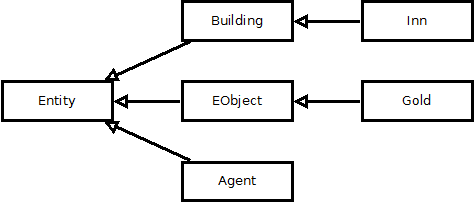
\includegraphics[width=.7\textwidth]{diagramaDeClasesEntidades}

 \caption{Diagrama de clases de las entidades}
 \label{fig:diagramaDeClasesEntidades}
\end{figure}

Cada elemento del mundo relevante para el juego, el cual es mantenido por Unity
como un \texttt{GameObject}, tiene asociado siempre un objeto de una de las
clases que se muestran en la figura (que no sea abstracta). 
Vale mencionar a su vez que la clase \texttt{Entity} hereda de
\texttt{MonoBehaviour}, por lo que todos las entidades pueden implementar los
métodos \texttt{Update}, \texttt{Start}, \texttt{Awake}, etc., facilitando el
manejo de las objetos físicos desde el código propio del sistema. 
Los elementos no relevantes para el sistema no tendrán una de estas clases
asociada. 
Éstos serán las paredes, árboles, terreno, entre otros.

\subsection{Clases de las entidades}

Toda entidad física tendra asociada una clase que herede de \texttt{Entity}. 
Por esto, en esta clase se encuentran algunas propiedades comunes (como la
descripción de la entidad, su nombre, posición, etc.), así como métodos comunes
a todas las entidades.

Los elementos que no son agentes pero sí son móviles serán representados por la
clase \texttt{EObject}. 
Actualmente, sólo existe una implementación de esta clase abstracta, la cual es
\texttt{Gold}, que representa los tesoros que pueden levantar los agentes.

Las clases que hereden de \texttt{Building} representarán edificios en el mundo.
Tendrán la característica de ser elementos grandes, a los cuales los agentes
podran ingresar, o sea, representan un volumen en el mundo. 
Físicamente son representados por un \texttt{GameObject} sin \texttt{Collider}
ni textura, con forma de ortoedro. 
Por esto, puede representar una zona en el mundo.

La implementación actual de esta clase es \texttt{Inn}, el cual representaría un
hotel. En el juego de prueba actual, se puede observar un objeto vacío como fue
descripto, el cual está rodeado por paredes. Éstas simplemente representan
obstáculos para el agente, pero no mantiene información asociada ni objeto de
tipo \texttt{Entity}.  A un \texttt{Building} se le puede consultar por si una
determinada posición se encuentra dentro o fuera de ella, siendo ésta su
principal función.

Finalmente, la clase más importante para el sistema es \texttt{Agent}. Esta
maneja toda la información relacionada al agente con respecto al juego (esto es
vida, elementos que lleva en un mochila, velocidad a la que se puede mover,
etc). A su vez, implementa todos los métodos necesarios para su manejo. Entre
estos se encuentran la generación de la percepción del agente, y todas las
acciones que puede realizar. Éstos se verán en mayor detalle en la sección
\ref{sec:agentes}.

\subsection{Terreno}

El terreno físicamente es un terreno común de Unity. Para poder ser utilizado
por los agentes, el terreno tiene asociado un grafo con forma de grilla. Ésta
está formada por un conjunto de nodos, los cuales tienen una posición asociada,
y un conjunto de aristas, las cuales representan las conexiones entre los nodos.
Cualquier posición del terreno es válido, tanto para los agentes como para el
resto de las entidades, pero a la hora de generar la percepción, éstos serán
asociados con el nodo más cercano a la posición en la que se encuentran. El
grafo es generado gracias a un \textit{plugin} realizado por \textit{Aron
Granberg}, llamado \textbf{A* Pathfinding Project} \footnote{Para más
información sobre este proyecto, dirigirse
a \url{http://arongranberg.com/astar/features}}.

\subsection{Agentes}

\label{sec:agentes}

En esta sección se describirán más detalladamente las características de los
agentes, sus propiedades y métodos.

El agente tiene como propiedades la vida actual y máxima, los elementos
(\texttt{EObject}) que lleva en la mochila, la velocidad máxima que puede
alcanzar al moverse, la profundidad de visión (es una magnitud de distancia, que
representa la máxima distancia a la que se pueden encontrar los objetos que el
agente puede percibir), y el alcance del agente (la máxima distancia que pueden
tener los objetos si el agente quiere levantarlos).

\subsubsection{Percepción}

Los agentes son las únicas entidades que pueden solicitar percepciones. Una
percepción es un conjunto de elementos que pueden ser percibidos, que se
encuentran dentro de un radio predeterminado para cada agente. Estos elementos
pueden ser tanto otras entidades como los nodos. Cada uno de estos elementos
luego es consultado por las caracteristicas que son de interés para el agente,
lo que es devuelto en el formato en el que se envia la percepción al agente.
A su vez, la percepción también incluye información propia del agente que no es
visible por otros agentes en su propia percepción, como la vida, o los elementos
que lleva en su mochila.

Más específicamente, existe una interfaz llamada \texttt{IPerceivableEntity}, la
cual es implementada por todas aquellas clases que puedan ser percibidos, cuya
única característica es que tienen un método que devuelve la representación
final de ese objeto para ser luego enviado dentro de la percepción. Como se
explico antes, estas son las entidades y los nodos. Con respecto a los nodos, al
estar utilizando el plugin \textbf{A* Pathfinding Project}, se decidió realizar
una \textit{cáscara}, esto es, una clase que contiene en una propiedad a una
variable de tipo \texttt{GridNode}, que es la clase provista por dicho
\textit{plugin} para representar a los nodos. Esta clase hereda de
\texttt{IPerceivableEntity}, por lo que implementa el método que genera la
representación final del nodo. La clase \texttt{Entity} también hereda de
\texttt{IPerceivableEntity}, por lo que toda clase de la jerarquía de clases de
la Figura \ref{fig:diagramaDeClasesEntidades} lo implementa.

La manera de percibir las entidades es a través de la utilización de la función
\texttt{OverlapSphere}, la cual detecta todos los \texttt{Collider} que se
encuentran dentro de una determinada esfera, la cual es casteada en la posición
del agente con un determinado radio, el cual es la profundidad de visión. Esta
función devuelve una lista con dichos colliders, los cuales se chequea que sean
del tipo buscado, y se obtiene su objeto de clase \texttt{Entity} asociado. 

Para los nodos, se hace un recorrido \textit{primero en anchura} sobre los
nodos, partiendo del nodo más cercano al agente, hasta una determinada
profundidad. Luego se chequea si las posiciones de los nodos se encuentran
dentro del rango visible.

\subsubsection{Acciones}

Actualmente las acciones posibles para los agentes son:

\begin{itemize}
\ttfamily
\item noop
\item move
\item pickup
\item drop
\end{itemize}

Las acciones pueden tener parámetros, y tienen un conjunto de precondiciones
y postcondiciones que se chequean y ejectuan en el momento que son recibidas por
el sistema. Ésto se observa en el código del agente, más precisamente en la
clase \texttt{Agent}, donde por cada acción hay dos métodos, los cuales
determinan las precondiciones y las postcondiciones.

\texttt{noop} es la acción nula, por lo que no genera ningún efecto, y puede ser
aplicada en cualquier momento. \texttt{move} es la acción de movimiento, que
recibe como parámetro el nombre del nodo al cual debe moverse, y cuya
precondición es que el agente se encuentre en un nodo adyacente a éste.

\texttt{pickup} tiene como precondición que el identificador de objeto que es
pasado por parámetro sea un objeto válido, y que se encuentre dentro de un radio
determinado. Este radio es mayor al tamaño de los nodos, por lo que encontrarse
en el mismo nodo que el objeto alcanza para que el agente pueda levantar el
objeto. Como postcondición, se agrega el objeto al \textit{backpack} del agente,
y se deshabilita su \texttt{GameObject}.

Finalmente, \texttt{drop} tiene como precondición que el identificador de objeto
pasado por parámetro sea un objeto válido que se encuentre en el
\textit{backpack} del agente.  Su postcondición es que el objeto vuelva a ser
habilitado, se cambia su posición a la actual del agente, y se le agrega una
determinada fuerza para que el objeto se mueva fuera de la posición del agente.

\section{Futuras modificaciones}

El sistema fue pensado para que sea fácil agregar nuevos clases dentro del
esquema planteado, así como nuevas acciones. Sin embargo, el principal trabajo
a realizar se encuentra en el diseño de un mundo que pueda generar un interés
desde el punto de vista del estudio de los sistemas multi-agente, el cual cumpla
con las condiciones planteadas por el sistema, como su espacio tridimensional
y su manejo del ciclo de acción y percepción en tiempo real. 

\section{Conclusión}

El desarrollo del sistema conllevó un arduo trabajo sobre una plataforma que
presenta sus beneficios en el área del desarrollo ágil de juegos, pero que sin
embargo presenta también sus limitaciones en el uso de herramientas externas,
o principalmente en el uso de estrategias de desarrollo fuera de su propuesta,
a pesar de soportar sí lenguajes y una \textit{API} poderosos. Al haber estado
fundamentalmente desarrollando del lado del motor de un juego, nos vimos
teniendo dificultades por no seguir con el modo de desarrollar juegos que
propone \textbf{Unity 3D}. Por esto quedó un diseño desacoplado entre motor de
conexión con los agentes, y la representación y simulación del mundo.

De cualquier manera, creemos que la etapa de luchar contra estos problemas ya
pasó, ya que los próximos pasos a realizar no dependen de las modificaciones en
la arquitectura básica del sistema, sino de la implementación de un sistema
multi-agente por encima de lo provisto. Por esto, esperamos que sea fructífera
la planeada aplicacación del sistema en la cátedra de Inteligencia Artificial,
para poder observar el producto de nuestro trabajo en funcionamiento.

\end{document}

